%%%%%%%%%%%%%%%%%%%%%%%%%%%%%%%%%%%%%%%%%
% Beamer Presentation
% LaTeX Template
% Version 1.0 (10/11/12)
%
% This template has been downloaded from:
% http://www.LaTeXTemplates.com
%
% License:
% CC BY-NC-SA 3.0 (http://creativecommons.org/licenses/by-nc-sa/3.0/)
%
%%%%%%%%%%%%%%%%%%%%%%%%%%%%%%%%%%%%%%%%%

%----------------------------------------------------------------------------------------
%	PACKAGES AND THEMES
%----------------------------------------------------------------------------------------

\documentclass[aspectratio=169,usenames,dvipsnames]{beamer}

\usepackage[utf8]{inputenc}
\usepackage{booktabs}
\usepackage{tabularx}
\usepackage[authordate,bibencoding=auto,strict,backend=biber,natbib]{biblatex-chicago}
\addbibresource{bib.bib}
\usepackage{graphicx}
% \hypersetup{
%     colorlinks,
%     %citecolor=black,
%     linkcolor=black
% }
\usepackage{array}
\usepackage{caption}
\usepackage{threeparttable}
\usepackage{epigraph} 
\usepackage{lscape}
\usepackage{adjustbox}
\newcommand*{\Scale}[2][4]{\scalebox{#1}{\ensuremath{#2}}}%
\usepackage{import}
\newenvironment{wideitemize}{\itemize\addtolength{\itemsep}{10pt}}{\enditemize}
\usepackage{amsmath}
\usepackage{csvsimple}
\usepackage{siunitx}
\usepackage{filecontents}
\usepackage{rotating}
\usepackage{multirow}
\usepackage{amsmath}
\usepackage{subcaption}
\usepackage{appendixnumberbeamer}
\usepackage{float}
\usepackage{amsmath}
\usepackage{csvsimple}
\usepackage{hyperref}
\newtheorem{proposition}{Proposition}
\usepackage{xcolor}
\def\boxit#1#2{%
    \smash{\color{red}\fboxrule=1pt\relax\fboxsep=2pt\relax%
    \llap{\rlap{\fbox{\phantom{\rule{#1}{#2}}}}~}}\ignorespaces
}
\newenvironment{variableblock}[3]{%
  \setbeamercolor{block body}{#2}
  \setbeamercolor{block title}{#3}
  \begin{block}{#1}}{\end{block}}
\usepackage{appendixnumberbeamer}
\usepackage{tikz,pgfplots}
\usepackage{tkz-fct}
\usepackage{amsthm}
\pgfplotsset{compat=1.10}
\usepgfplotslibrary{fillbetween}
\mode<presentation> {
\AtBeginSection[]
{
    \begin{frame}
        \frametitle{Table of Contents}
        \tableofcontents[currentsection]
    \end{frame}
}
% The Beamer class comes with a number of default slide themes
% which change the colors and layouts of slides. Below this is a list
% of all the themes, uncomment each in turn to see what they look like.

\usetheme{default}
%\usetheme{AnnArbor}
%\usetheme{Antibes} -
%\usetheme{Bergen}
%\usetheme{Berkeley}
%\usetheme{Berlin}
%\usetheme{Boadilla}
%\usetheme{CambridgeUS}
%\usetheme{Copenhagen} -
%\usetheme{Darmstadt}
%\usetheme{Dresden}
%\usetheme{Frankfurt}
%\usetheme{Goettingen}
%\usetheme{Hannover}
%\usetheme{Ilmenau}
%\usetheme{JuanLesPins}
%\usetheme{Luebeck}
%\usetheme{Madrid}
%\usetheme{Malmoe}
%\usetheme{Marburg}
%\usetheme{Montpellier}
%\usetheme{PaloAlto}
%\usetheme{Pittsburgh}
%\usetheme{Rochester} -
%\usetheme{Singapore}
%\usetheme{Szeged}
%\usetheme{Warsaw}

% As well as themes, the Beamer class has a number of color themes
% for any slide theme. Uncomment each of these in turn to see how it
% changes the colors of your current slide theme.

%\usecolortheme{albatross}
%\usecolortheme{beaver}
%\usecolortheme{beetle}
%\usecolortheme{crane}
%\usecolortheme{dolphin}
%\usecolortheme{dove}
%\usecolortheme{fly}
%\usecolortheme{lily}
%\usecolortheme{orchid}
%\usecolortheme{rose}
%\usecolortheme{seagull}
%\usecolortheme{seahorse}
%\usecolortheme{whale}
%\usecolortheme{wolverine}

%\setbeamertemplate{footline} % To remove the footer line in all slides uncomment this line
%\setbeamertemplate{footline}[frame number] % To replace the footer line in all slides with a simple slide count uncomment this line
\setbeamertemplate{theorems}[numbered]
\setbeamertemplate{navigation symbols}{} % To remove the navigation symbols from the bottom of all slides uncomment this line
}
\setbeamertemplate{caption}{\raggedright\insertcaption\par}
  \setbeamertemplate{enumerate items}[default]
  %\setbeamertemplate{page number in head/foot}{\insertframenumber}
\usepackage{graphicx} % Allows including images
\usepackage{booktabs} % Allows the use of \toprule, \midrule and \bottomrule in tables
%\usepackage {tikz}
\newtheorem*{theorem*}{Theorem}
\newtheorem*{lemma*}{Lemma}
\newtheorem*{proposition*}{Proposition}
\newtheorem*{corollary*}{Corollary}
\newtheorem*{definition*}{Definition}
\DeclareMathOperator*{\argmin}{arg\,min}
\newtheorem*{assumption}{Assumption}
\usetikzlibrary {positioning}
\renewcommand{\arraystretch}{1.5}
\newcommand\hideit[1]{%
  \only<0| handout:1>{\mbox{}}%
  \invisible<0| handout:1>{#1}}
\usepackage[default]{lato}

\setbeamercolor{block body alerted}{bg=alerted text.fg!10}
\setbeamercolor{block title alerted}{bg=alerted text.fg!20}
\setbeamercolor{block body}{bg=structure!10}
\setbeamercolor{block title}{bg=structure!20}
\setbeamercolor{block body example}{bg=green!10}
\setbeamercolor{block title example}{bg=green!20}


\makeatletter
\let\save@measuring@true\measuring@true
\def\measuring@true{%
  \save@measuring@true
  \def\beamer@sortzero##1{\beamer@ifnextcharospec{\beamer@sortzeroread{##1}}{}}%
  \def\beamer@sortzeroread##1<##2>{}%
  \def\beamer@finalnospec{}%
}
\makeatother
%\usepackage {xcolor}

%----------------------------------------------------------------------------------------
%	TITLE PAGE
%----------------------------------------------------------------------------------------

\title[diss]{Lecture 11: Promotions as Tournaments} % The short title appears at the bottom of every slide, the full title is only on the title page
\author{Compensation in Organizations} % Your name
\institute[shortinst]{Jacob Kohlhepp}
\date{\today} % Date, can be changed to a custom date

\begin{document}

\begin{frame}
\titlepage % Print the title page as the first slide

\end{frame}


\begin{frame}{Performance Pay is Not the Norm}

\begin{wideitemize}
    \item 2/5 of hours worked were in jobs with performance pay 
    %https://journals.sagepub.com/doi/full/10.1177/002795011322600102?casa_token=94SHmpkCkPcAAAAA%3AANoUOfd1PrHF593u0TyNBwFeEJQLfkWzDW1uzSiaWKUVimv8OeumcxraEncSI9E15MYs4ai8knN7
    \item Performance pay is more common in some industries and not others.
    \item It has been declining over time.
    \item How can firms encourage effort without explicit incentives?
\end{wideitemize}
    
\end{frame}


\begin{frame}
\centering
    \huge Big Question:  What motivates people to work hard when they are paid a flat salary?
\end{frame}

\begin{frame}{The Logic of Performance Pay}
\begin{wideitemize}
    \item \textbf{Performance Pay:} More pay when you put in more effort (on average)
    \begin{wideitemize}
        \item I work hard to make more at my current job!
    \end{wideitemize}
\end{wideitemize}

\end{frame}

\begin{frame}{Three Alternatives}

\begin{wideitemize}
    \item We will study three alternative ways to encourage performance.
    \item \textbf{Relational Contracts:} The possibility of termination.
    \begin{wideitemize}
        \item I work hard to keep my job!
    \end{wideitemize}
    \item \textbf{Career Concerns:} The possibility of getting a better job at a different firm.
    \begin{wideitemize}
        \item I work hard to get a better future job!
    \end{wideitemize}
    \item \textbf{Tournaments/Promotions:} The possibility of getting a better job at my current firm.
    \begin{wideitemize}
        \item I work hard to get promoted!
    \end{wideitemize}
\end{wideitemize}
    
\end{frame}


\begin{frame}{Changing CEOs at GE}

\begin{wideitemize}
    \item In 2000, Jeffrey Immelt was a VP at General Electric with  a salary of \$1 million.
    \item In 2001, Jack Welch retired as CEO of General Electric.
    \item Jeffrey Immelt then became CEO, and made \$2.75 million his first year.
    \item Discussion: Did the value of Immelt's skills increase 3 times in 1 year?\pause
    \item The job of CEO was itself a form of prize or reward.
\end{wideitemize}
    
\end{frame}


\begin{frame}
\centering
    \huge I may work hard to get a better job at my current company!

\end{frame}

\begin{frame}{CEO Pay}

\begin{wideitemize}
    \item CEOs already have the biggest prize in the promotion tournament.
    \item Therefore if tournament theory holds weight, they must be compensated in other ways.
    \item CEOs are indeed paid in large part via bonuses and stock options.
    \item This is more similar to traditional performance pay.
\end{wideitemize}
    
\end{frame}


\begin{frame}{Verbal Model: Tournaments}
\begin{wideitemize}
    \item Suppose there are two workers and one firm.
    \item Worker output is effort plus some noise/luck: $y_i=e_i + \epsilon_i$
    \item Effort has cost $c(e)$
    \item The firm gives a ``prize" $w$ to whoever has the highest output.
    \item Workers exert effort in order to increase the probability they get the prize:
    \[\max_{e_1} w \cdot Pr(e_1 + \epsilon_1\geq e_2 + \epsilon_2) - c(e_1)\]
    \item The chance of winning plays the role of $\beta$ and motivates workers to exert effort.
\end{wideitemize}
    
\end{frame}

\begin{frame}{Tournaments vs. Promotions}

\begin{wideitemize}
\item We did not specify what $w$ was.
\item We only required that the workers care about it.
\item It could be an actual cash prize/bonus...
\pause
    \item Or a promotion.
    \item What is crucial is that there is competition: only the person who produces the most gets it!
    \item This introduces some new issues.
\end{wideitemize}
    
\end{frame}
\section{Issues with Tournaments}

\begin{frame}{Bandiera, Barankay, and Rasul (2005)}

\huge A leading farm in the UK switched from relative pay to piece rates.

    
\end{frame}

\begin{frame}[c]{Bandiera, Barankay, and Rasul (2005)}
\centering
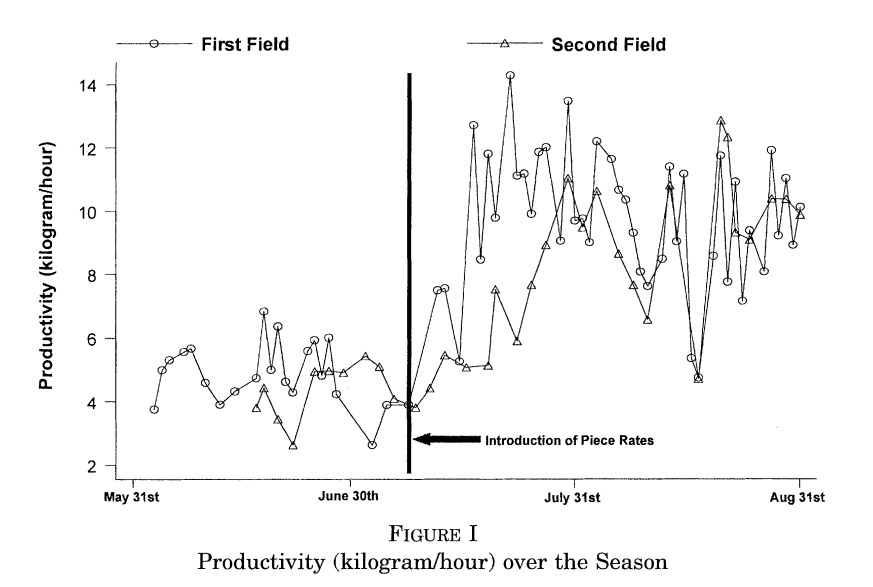
\includegraphics[width=0.85\textwidth]{pictures/switched_time_tournament.png}

    
\end{frame}

\begin{frame}[c]{Bandiera, Barankay, and Rasul (2005)}
\centering
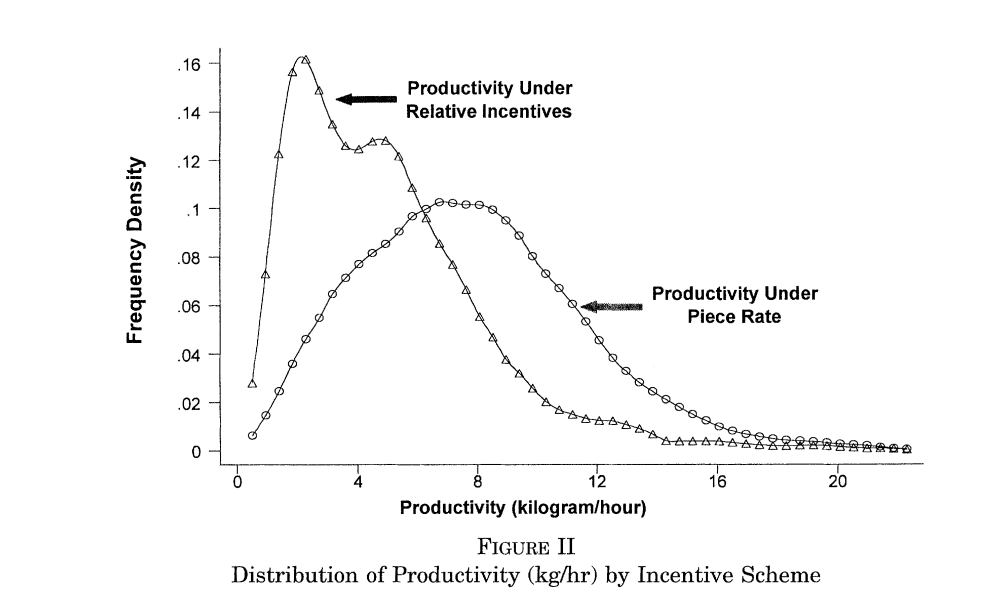
\includegraphics[width=0.85\textwidth]{pictures/switched_density_tournament.png}

    
\end{frame}

\begin{frame}[c]{Bandiera, Barankay, and Rasul (2005)}
\centering
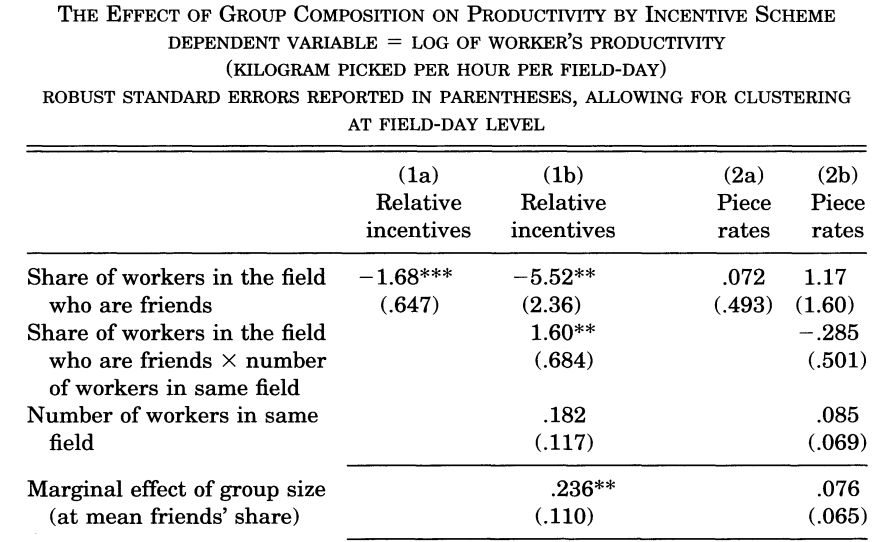
\includegraphics[width=0.85\textwidth]{pictures/friends_tournaments.png}

    
\end{frame}

\begin{frame}{Bandiera, Barankay, and Rasul (2005)}
    \begin{wideitemize}
        \item Is the friends result because people are altruistic?
        \begin{wideitemize}
            \item I want my friends to get paid more.
        \end{wideitemize}
        \item Or is it because of collusion?
        \begin{wideitemize}
            \item My friends and I work together to get more from the system?
        \end{wideitemize}
        \item It turns out that the fruit company grew two types of fruit.
        \begin{wideitemize}
            \item Fruit that grows in 6-7 foot dense shrubs (Type 2) where it is hard to see coworkers.
            \item Fruit that grows in such a way where it is easier to see coworkers (Type 1)
        \end{wideitemize}
        \item If this monitoring channel matters, this suggests collusion. If not, this suggests altruism.
    \end{wideitemize}
\end{frame}

\begin{frame}[c]{Bandiera, Barankay, and Rasul (2005)}
\centering
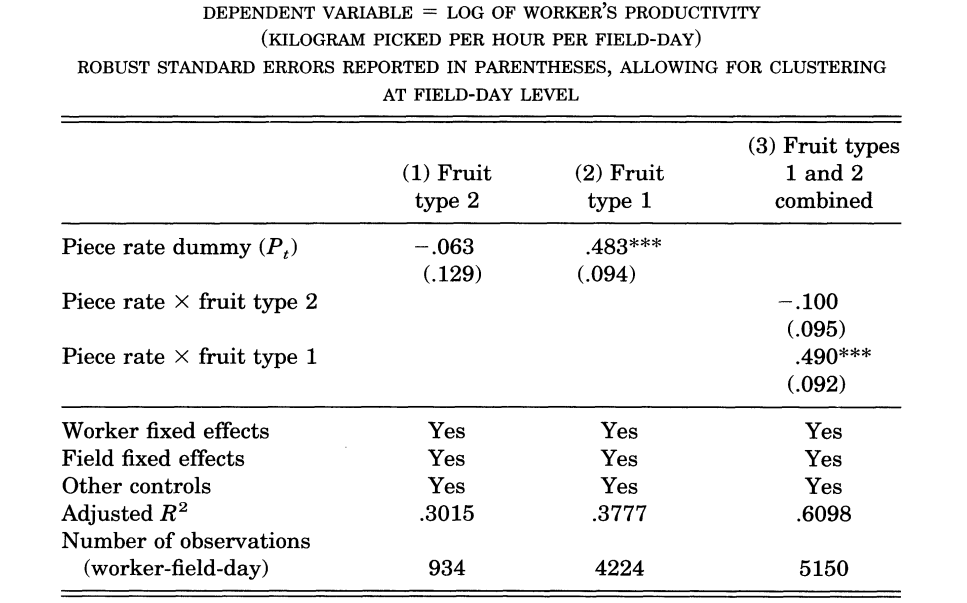
\includegraphics[width=0.85\textwidth]{pictures/switched_fruittype_tournaments.png}

    
\end{frame}

\begin{frame}{Can Collusion be Prevented? Another Example}
\begin{wideitemize}
    \item Chickens raised for meat are often grown by contractors.
    \item These growers are often paid via a tournament.
    \item There is a threat of collusion because growers are located near each other.
    \item One method used to combat this is to rotate who competes with who.
    \item Broilers (the main company) does this by changing the delivery schedule.
\end{wideitemize}

\hfill Source: ``A Real Game of Chicken," Knoeber (1989)
\end{frame}



\begin{frame}{Intrinsic Differences in Productivity}
    \begin{wideitemize}
        \item Our model assumed both workers had the same base productivity.
        \item But what if one worker is just more productive at every level of effort?
        \item The less skilled worker then may exert no effort because they have no chance.
        \item Knowing this, the more skilled will also exert no effort.
    \end{wideitemize}
\end{frame}
\begin{frame}[c]{The Peter Principle}
\centering
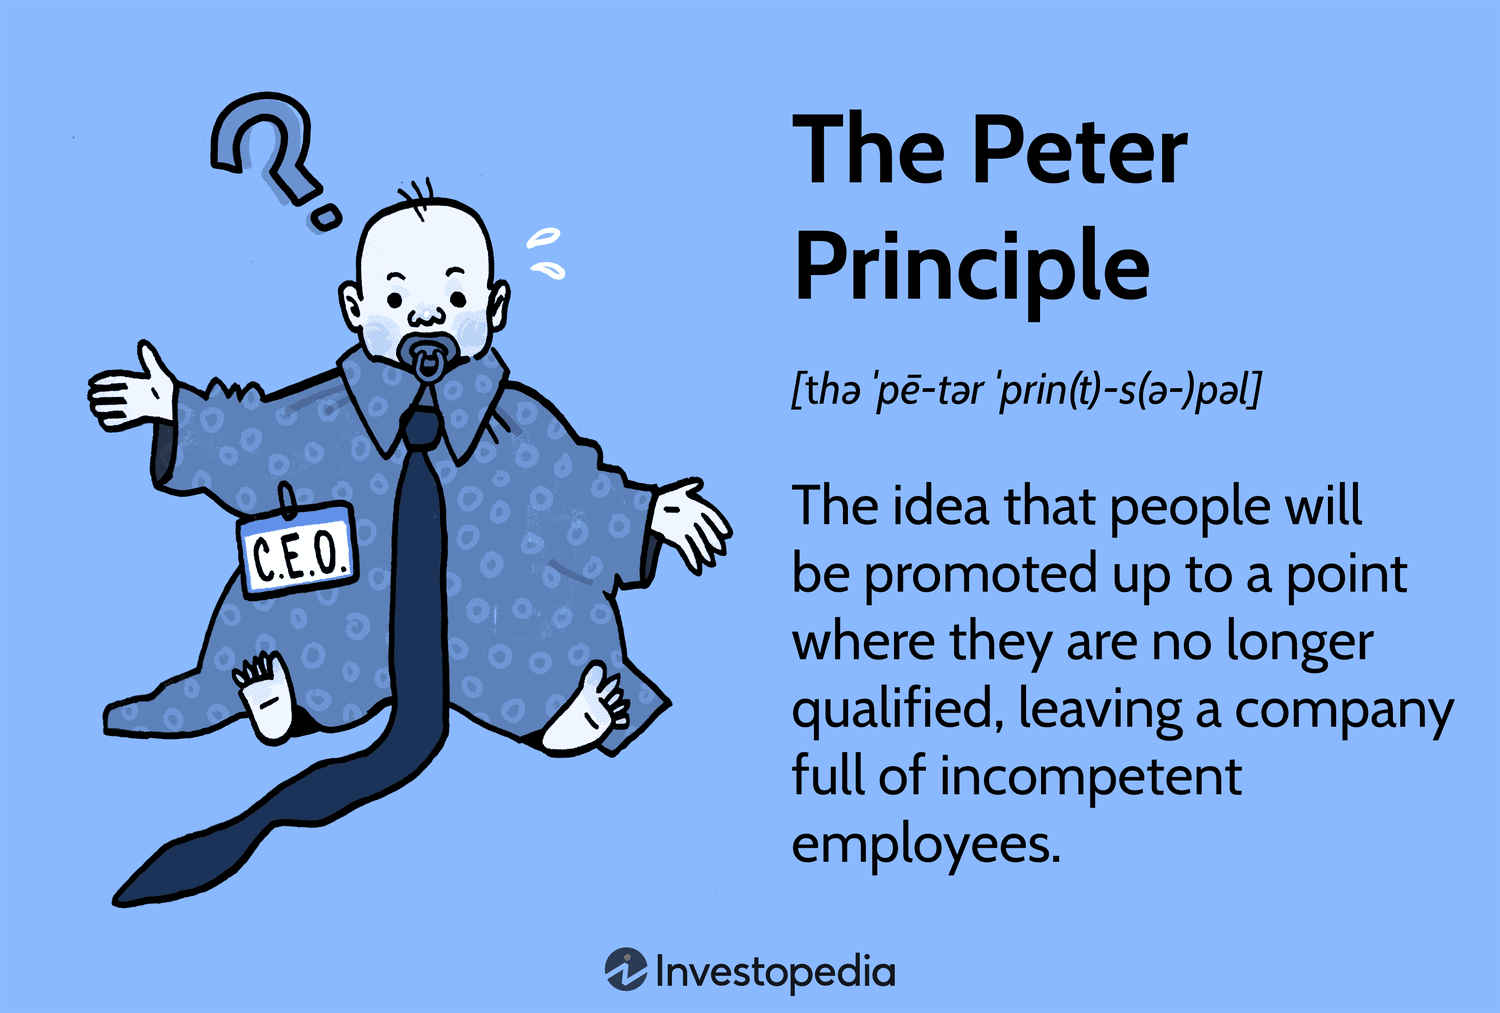
\includegraphics[width=0.8\textwidth]{pictures/peter-principle.asp-final-556adb51ee7f45098cbd12bb1ce4f44e.png}
    
\end{frame}



\begin{frame}{The Peter Principle}
\begin{wideitemize}
    \item We have shown that firms can use tournaments to encourage effort.
    \item But if promotions are the prize, then people are promoted based on performance at a different job.
    \item Example: becoming CEO because I am good at accounting.
    \item This suggests a trade-off between using jobs as prizes and using them as actually productive functions.
    \item Whether this trade-off is real depends on whether jobs fundamentally change as you move up.
    \item In economic consulting, analysts program and partners solicit clients.
    \item There is some empirical evidence of this (Acosta 2010)
\end{wideitemize}
\end{frame}

% \begin{frame}{Sabotage}
% \begin{wideitemize}
%     \item The performance of coworkers impacts pay as much as own performance.
%     \item There may be an incentive to sabotage others, or at a minimum not help others.
%     \item In highly interdependent work this can be disastrous.
%     \item This is similar to gaming and multitasking concerns.
% \end{wideitemize}
% \hfill Source: ``Pay Equity and Industrial Politics," Lazear (1989)
% \end{frame}


\begin{frame}{Promotions Discourage Helping Others: Drago and Garvey (1998)}
\begin{wideitemize}
    \item A survey of 938 Australian employees.
    \item A researcher visited each workplace and identified who worked together.
    \item Two people are said to be in a work group if they worked at the same workplace, the same occupation and in close physical proximity while performing most tasks.
    \item The paper proxies for a promotion or prize as the spread in wages within a group.
    \item They find that larger prizes (which they interpret as bigger promotions) reduce worker's ``helping efforts."
    \item The reduction is both economically and statistically significant.
\end{wideitemize}
    
\end{frame}

% \begin{frame}{Collusion}
% \begin{wideitemize}
%     \item Only relative performance matters.
%     \itme Therefore if you and I are in a tournament, we can both agree to exert 0 effort and split the prize.
%     \item This helps workers at the expense of the firm.
%     \item But it requires some form of commitment: if I know you are exerting 0, I am tempted to work just a little bit and get everything rather than split.
%     \item Therefore collusion is more likely when there is repeated interaction between workers or pre-existing relationships.
% \end{wideitemize}
% \end{frame}





\end{document}




